\documentclass{article}
\usepackage[utf8]{inputenc}
\usepackage{fancyhdr}
\usepackage{graphicx}
\usepackage{biblatex}
\addbibresource{bib.bib}

\title{\textit{When do armed revolts succeed: lessons from Lanchester theory} by M. Atkinson et al.: en expository review}
\author{Karington Kim, Catie Lamberson, Harrison Stanton}
\date{May 4, 2022}

\begin{document}

\maketitle

\begin{center}
\bf{Abstract}
\end{center}
\textit{When do Armed Revolts Succeed: Lessons From Lanchester Theory} by M. Atkinson et. al is an original research model in Operations Research that tries to determine whether or not a revolt will succeed. The authors propose a new model of such revolts that describes their evolution by building on the classic Lanchester theory of combat, which states that a military forces’s losses will be directly tied to the size of the opposing force. The new model accounts for the split in the population between those loyal to the regime and those favoring the rebels. The authors show that, unlike the original Lanchester model, the outcome of a revolt is independent of the initial force sizes; it only depends on the fraction of the population supporting each side and how well they actually fight. The model's predictions are consistent with the situations observed in Afghanistan, Libya and Syria (September 2011).


\section{The Journal and Authors}
The article When Do Armed Revolts Succeed: Lessons from Lanchester Theory[1] is an article of original research in the field of operational research. It was published in October 2011 in the Journal of Operational Research Society, it is a peer reviewed journal on the subject of Operations Research and Management. It specializes/emphasizes in illustrating real applications, technical approaches and a variety of environments. It especially deals with applications of OR. The journal publishes 22 issues per year and it has an impact factor of 2.175(2019). The article is co-authored by:
\begin{itemize}
    \item MP. Atkinson
    \item A. GutFraind
    \item M. Kress
\end{itemize}
MP. Atkinson’s research interests include stochastic processes, computational methods, and military operations research and is an Assistant Professor of Operations Research at the Naval Postgraduate School. 
A. GutFraind’s research interests are in complex networks and systems, public health, epidemiology of infectious diseases, mathematical models of security.
M. Kress’s research interests are military operations research, combat modeling, and military logistics. He is a professor of Operations Research at the Naval Postgraduate School.

\section{The article}
\subsection{Background, purpose, scope}
The article When Do Armed Revolts Succeed: Lessons from Lanchester Theory is in the area of Military Operations Research, which studies problem-solving and decision-making that helps manage organizations usually under the conditions of scarce resources. The authors assume that readers are familiar with the following terms used in military operations research:
\begin{itemize}
    \item \textbf{Lanchester Model.} Refers to the formulas in math, modeled using differential equations, that show the strengths of military forces.
    \item \textbf{Armed Revolt.} Refers to two forces that rely on manpower, intelligence, and other resources.
    \item \textbf{Attrition Rate.} Refers to the gain rate of the attacker.
    \item \textbf{LSER.} Refers to the liberation-subjugation effectiveness ratio of an armed revolt
    \item \textbf{Indirect Intervention.} Refers to the provision of military or political assistance to a force in the revolt.
\end{itemize}
This article focuses specifically on building on the Lanchester theory. The models for the Lanchester theory are formulas for calculating the relative strengths of military forces. They use differential equations to describe the dependence of two armies’ strengths as a function of time\cite{atkinson2012armed}.
\\The scope of the research is twofold:
\begin{enumerate}
    \item This research gives a realistic outcome to these revolts that a usual Lanchester model does not.
    \item It also studies the results of foreign intervention. Is it best for someone to intervene and at what level?
\end{enumerate}
The results of this study, that contrary to Lanchesterian models and insights, the result of a revolt is not dependent on force size. It only depends on the size of the population that supports each side.
\medskip
\\Specifically, the authors want to describe how the revolts might evolve by building off of the Lanchester theory. They want to explicitly prove the assumptions of previous models. They hope their model can help anticipate the outcomes of future revolts.
\subsection{Literature review and originality}
The results from this article are original. However, this article adds onto and takes inspiration from previous studies using the Lanchester Linear Law and Deitchman’s guerrilla warfare model.
\begin{itemize}
    \item In 1962, Deitchman published the article A Lanchester model of Guerrilla Warfare\cite{deitchman1962lanchester}, and in 1968, Schaffer published the article Lanchester Models of Guerrilla Engagements\cite{schaffer1968lanchester}. These both more accurately described the Guerrilla Warfare Model. This model uses the Lanchester equations that describe guerrilla warfare. It doesn’t only depend on government forces, but on the size of the guerrilla force. This was one of the first articles to study different population sizes in war and how they impact the outcome.
    \item In 2009, Washburn and Kress published the article Combat Modeling\cite{washburn2009combat}, where they created and described the Lanchester Linear Law. This gives further explanation and application to the Lanchester model. The Lanchester Linear Law applies to unaimed fire into enemy territory and the results of this depend on the target area.
\end{itemize}
These articles gave definition to this study. In this study, they look at conflict between forces when the population has a role. However, unlike most studies on the Lanchester model that believe that the outcome of a battle is based on force size, they look at the control of friendly and hostile populations. The authors believe the outcome of a revolt is based on support in the population more than force size, for this reason, that is the main study of this article. With the model from this article, the end revolt and stalemate situations are identified and it studies the effects of foreign intervention and support of the population.
\medskip
\\This model shows that as opposed to most Lanchesterian force-on-force studies, the outcome is not dependent on initial force size.
\medskip
\\The shortfall of these previous models is that they do not consider the friendly and hostile population. Yet, recent studies (such as Kress and Szechtman in their Why Defeating Insurgencies is Hard: The Effect of Intelligence in Counterinsurgency Operations-A Best-Case Scenario(2009)\cite{kress2009defeating}) hypothesize that there is an impact of population on the revolts. They focused on: 
\begin{enumerate}
    \item collateral damage,
    \item how intelligence alters the dynamics.
\end{enumerate}
In particular, population has proven to be an important variable in the study. Because depending on whether or not the population is supportive or hostile changes the outcome of the revolt.
\medskip
\\The authors identified this research gap and built this model for hostile versus friendly populations. This is the first time that this has been done with the Lanchester model, making their model original. The authors hypothesize that this improvement will significantly improve research using this model and will help anticipate the outcomes of different kinds of revolts.
\subsection{Data}
The authors did collect some data on their own, and they got data from the following sources: 
\begin{itemize}
    \item Table 1 shows the correlation between research on past armed revolts and their outcomes. These are all predictable by the model.
    \begin{figure}[htpb]
        \centering
        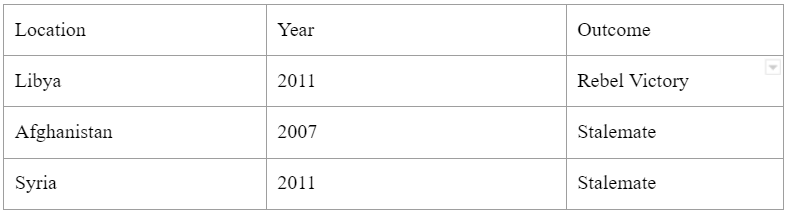
\includegraphics{datasample.png}
        \caption{Shows the research done in this article and the results that can be predicted by this model.}
        \label{Table 1}
    \end{figure}
\end{itemize}
\subsection{Methods}
The authors construct models to denote the fraction of the populations of supporters for both Blue (supporters) and Red (contrarians) and the fraction of the populations that are controlled by Blue and Red. Therefore, adding the fractions up should equate to 1. The authors notate that $X$ and $Y$ as fractions of the population $X$ controlled by $Y$. Therefore, the models are as follows:
\begin{itemize}
    \item $SB + SR = S$
    \item $CS + CR = C$
\end{itemize}
\medskip
\subsubsection{Modeling Assumptions}
The authors set various assumption throughout the study:
\begin{itemize}
    \item Support depends on unchanging factors such as tribal affiliation, social class, and ideology. Although this assumption was set initially, the authors also did allow leeway later on in the study to observe changes in behavior.
    \item The country is divided between Red and Blue, which would mean that a populated land that is lost by one force is gained by the other.
    \item Population in each region is homogeneous.
    \item Forces that fight over a region can be supported or opposed by the local population of that region.
    \item The following \textit{dominance assumptions} are made as well: $f_s>h_c$ and $f_c>h_s$.
\end{itemize}
\subsubsection{Variables and equations}
The authors use 6 variables in order to represent different populations: $S$, $C$, $B$, $R$, $X$, $Y$. The authors also denote $f_s$ and $f_c$ as the rates of liberation of friendly regions by Blue and Red. $h_c$ and $h_s$ denote the rates of subjugation of hostile regions by Blue and Red respectively.
\medskip
\\The differential equations are provided as follows:
\begin{itemize}
    \item $SB' = +f_sSB \cdot SR - h_sCR \cdot SB$
    \item $SR' = -f_sSB \cdot SR + h_sCR \cdot SB$
    \item $CR' = +f_cCR \cdot CB - h_cSB \cdot CR$
    \item $CB' = -f_cCR \cdot CB + h_cSB \cdot CR$
\end{itemize}
\medskip
\\Using these equations, the authors find that the conflict can result in one of three outcomes:
\begin{enumerate}
    \item \textit{Blue victory}: $SB + CB = 1$
    \item \textit{Red victory}: $CS + SR = 1$
    \item \textit{Stalemate}: Both sides control a fraction of total population.
\end{enumerate}
The authors define the attrition rate to be the gain rate of the attacker given by a scaling constant. The two outcomes of whether Blue or Red wins is dependent on the attrition ratio:
\begin{itemize}
    \item Blue wins if: $r_c < \frac{S}{1-S}$
    \item Red wins if: $r_s < \frac{1-S}{S}$
\end{itemize}
However, a stalemate occurs when neither of these two outcomes are met. At this point, the authors extend their basic model to include foreign intervention and shift of popular support. Foreign intervention includes both direct and indirect intervention. Direct intervention involves factors such as NATO entering the situation or air support. Indirect interventions is defined as being given force multipliers such as intelligence, training, logistical support, and advanced weapons. It is assumed that only one side will receive this intervention. 
\medskip
\\In the case of a direct intervention, the authors defined a new variable $\lambda$ as the combat power of the foreign intervention. With this new variable the original differential equations change as follows:
\begin{itemize}
    \item $SB' = +f_sSB \cdot SR - h_sCR \cdot SB + \lambda_sSR$
    \item $SR' = -f_sSB \cdot SR + h_sCR \cdot SB - \lambda_sSR$
    \item $CR' = +f_cCR \cdot CB - h_cSB \cdot CR - \lambda_cCR$
    \item $CB' = -f_cCR \cdot CB + h_cSB \cdot CR + \lambda_cCR$
\end{itemize}
\medskip
\\In the case of an indirect intervention, the force multiplier variable is introduced as $\mu$. Using this new variable, the authors found that in order for Blue to avoid defeat, the following condition must be met:
\begin{center}
    $\mu_s \ge \frac{1-S}{r_sS}$
\end{center}
\medskip
\\In order for Blue to secure a victory however, the following condition must be met:
\begin{center}
    $\mu_c > \frac{r_C(1-S)}{S}$
\end{center}

\subsection{Solution and Discussion}
The study found that there are three outcomes to any basic revolt situation, where there is no foreign intervention. The first situation is that the Supporters can fully wipe out the Contrarian force and regain total control of the region. In order for this to happen, the number of Supporters needs to be greater than the number of Contrarians times the rate at which the Contrarians can subjugate enemy territory, which is represented by the equation $r_{c} < S/(1-s)$ (represented by this equation). 
\medskip
\\The second situation that can occur is the Contrarians can completely wipe out the Supporters and maintain control over the entire region. The situation for this to happen is that the number of Contrarians needs to be greater than the number of supporters times the rate at which the supporters subjugate the Contrarians, as shown in the equation $r_{S} < (1-S)/S$.
\medskip
\\The third and final end scenario for an armed revolt is a stalemate, where the Contrarians occupy some amount of territory and the Supporters also occupy some amount of territory. This happens when neither of the above two conditions are met, and is also the most likely scenario.
\medskip
\\The authors represented these scenarios in Figure \ref{fig: random}. Graph A is a graph of one of the possible outcomes of their model, where $S = 40\%$. This graph models how the most likely scenario is actually a stalemate, where both sides occupy some territory. The graph also shows how it is more likely for the Red side, who is the original government, to achieve a victory than the Blue, or Contrarian, forces. Graph B depicts the territory that blue will occupy, again as a function of $r_{C}$ and $r_{S}$. 
\begin{figure}[h]
    \centering
    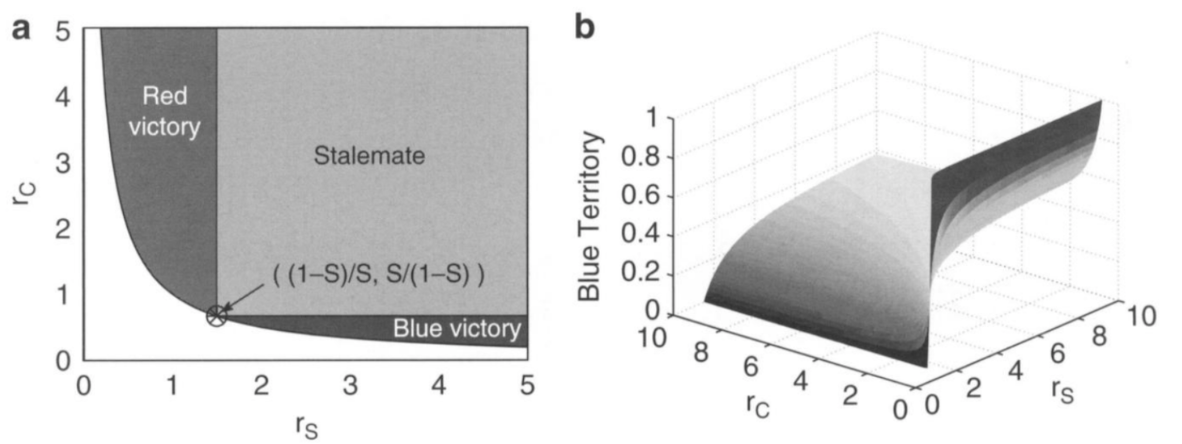
\includegraphics[scale = 0.35]{graphs.png}
    \caption{Model of the outcomes of an armed revolt as a function of $r_{S}$ and $r_{C}$}
    \label{fig: random}
\end{figure}
\medskip
\\
Another main finding of this study that is important to mention is that the initial sizes of the armies in question does not determine the outcome of the fight. Rather, the amount of people who actually support each side, even if they are not fighting, along with the effectiveness of each side at taking over enemy territory, are the factors that are going to determine which side wins the battle. This is the most different finding from the original Lanchester model, which indicates that size of each military is how to determine casualties and winners. 
\medskip	
\\The study additionally goes into more detail on more realistic military engagements, such as an armed revolt where another country actually aides one of the two sides. There are two situations that the authors modeled for. The first is indirect intervention, which includes policies such as embargoes and other political means to help one side. They included a force multiplier in the original equations that they produced for the basic situation to represent the help that the foreign country gives. What the study finds is that if the foreign country is helping the Supporters, the Supporters are more effective at defending their own territory, meaning they have more opportunity to attack the Contrarians and secure a victory.
\medskip
\\The second situation that is depicted in the article is when a foreign country offers direct intervention in support of the Supporters, such as air support. This direct support is actually largely effective, and eliminates any chance that the Contrarians could obtain a victory, leaving the only two possible outcomes as a stalemate or a Supporters victory. The reason that this happens is because the foreign help actually increases the Supporters ability to subjugate the enemy population. This is represented by a constant multiplied times the combat power of the Supporters. 
\medskip
\\In order to validate the results of their studies, the authors turned to Libya, Afghanistan, and Syria, which all had civil unrest and armed conflicts occurring in 2011. Their validation studies show the flaws in the concept of their model. The first flaw that presents itself is actually obtaining data. For all three events, they talk about how data that they need, such as whether or not the people support the armed revolt, is very difficult to obtain. This makes logical sense because it is going to be very difficult to interview people and get a big enough sample size to actually determine which side people support while there is a war happening. Because in most real life scenarios the authors cannot accurately obtain data, their model is has difficulty actually predicting what will happen in a conflict. While the model cannot obtain exact numbers and it struggles to be accurate enough to actually use in combat, their validation study showed how they can simulate the effect that policies implemented by governments will have. This is useful in determining the best ways to go about supporting one of the countries. The second problem that the validation study seems to point to is how specific of a situation the model is representing. For example, one of their countries they examined in their validation study was Syria, where the country was only experiencing civil unrest in which the military sometimes had to engage. 
\medskip
\\Because of their lack of data and examples, their validation study is weak in actually proving that their model is accurate to real life situations. The authors acknowledge that and mention how their model is an improvement over the original Lanchester model because they actually account for the possibility of a stalemate as an outcome. 
\subsection{Conclusion}
The article’s overall goal was to build a better model for warfare than the Lanchester model, which only accounted for the size of each force when determining who would win each military conflict. They did this by modeling the support each side had from the population, and how effective each side was at liberating their supporters and controlling more enemy territory. In order to build even further on that, the authors modeled help from foreign countries in the form of direct and indirect intervention. They found that the most important factor in determining the winner of a conflict was not the size of the military forces, but rather the support they had from the population $(S)$ and their attrition coefficients $(f_{C}$ and $h_{C})$ in enemy territory. The authors goal was to make it explicitly clear how policies and foreign action will affect combat. The authors say that in the future, a way to improve the model would be to make it effective in real time military conflict. 
\printbibliography


\end{document}
